\documentclass[11pt]{article}
\usepackage[margin=1in]{geometry}
\usepackage{fontspec}
\usepackage{graphicx}
\usepackage{booktabs}
\usepackage{amsmath}
\usepackage{caption}
\usepackage{float}
\usepackage{xcolor}
\usepackage{hyperref}
\graphicspath{{report/figures/}{figures/}}

\setmainfont{Latin Modern Roman}
\newfontfamily\devanagarifont[
    Path=/usr/share/fonts/google-noto/,
    UprightFont=NotoSerifDevanagari-Regular.ttf
]{Noto Serif Devanagari}
\newcommand{\hi}[1]{{\devanagarifont #1}}
\newcommand{\nep}[1]{{\devanagarifont #1}}
\newcommand{\piece}[1]{{\devanagarifont #1}}

\hypersetup{
    colorlinks=true,
    linkcolor=blue,
    urlcolor=blue,
    citecolor=blue
}

\title{LMA Individual Project --- Phase 1 Report \\
\large Data Collection and Tokenizer Construction \\
Hindi (Model H) and Nepali (Model L)}
\author{Gopal \\ 2023112006}
\date{August 19, 2026}

\begin{document}
\emergencystretch=2em
\maketitle

\section{Overview}
This report documents the Phase 1 data collection, preprocessing, splitting,
and tokenizer construction pipeline for two independent monolingual language
models: a higher-resource Hindi model (\textbf{Model H}) and a lower-resource
Nepali model (\textbf{Model L}). The two corpora, tokenizer training runs,
vocabularies, and evaluation artifacts are kept separate by language. No
pretrained tokenizer or shared vocabulary is used.

\section{Language Selection}

\subsection{Model H: Hindi}
Hindi was selected as the higher-resource language because it has a large
public digital footprint across news, literature, public-domain books,
magazines, and educational material. This made it a suitable anchor language
for Phase 1: enough data could be collected from many independent sources,
and the author's familiarity with Hindi will also support qualitative
generation checks in later phases.

\subsection{Model L: Nepali}
Nepali was selected from the permitted low-resource language list. It is
written primarily in Devanagari, which allowed the same script-aware crawler,
cleaner, and tokenizer infrastructure to be reused while still testing the
pipeline on a language that is lower-resource than Hindi. Because Hindi and
Nepali share a script, the corpus separation is enforced at the source level:
Hindi data is drawn from Hindi-specific domains and collections, while Nepali
data is drawn from Nepali domains and the Nepali portion of IndicCorp v2.

\section{Data Collection}

\subsection{Custom Crawler}
Manual/self-collected data was gathered with the custom crawler in
\texttt{crawler/}. The crawler performs recursive in-domain link traversal
from seed URLs, keeps a persistent SQLite frontier and visited-state database,
stores extracted document hashes, and supports resumable crawling across
sessions. The crawl policy used conservative throttling: up to 3 requests per
second per source configuration, bounded concurrency, retry limits, and
request timeouts. Sitemap and RSS fields are present in the source
configuration, and the crawler also supports PDF-oriented collection through
the surrounding extraction scripts.

HTML extraction uses \texttt{trafilatura} where available, with
BeautifulSoup/lxml-based parsing and cleanup as fallbacks. The extractor
removes scripts, styles, navigation residue, and repeated boilerplate before
the text is sent to the cleaning and filtering pipeline.

\subsection{Sources}
The Hindi corpus combines self-collected web and literary data with high-quality public domain collections. The largest Hindi self-crawled and literary sources include \texttt{hindwi}, \texttt{matrubharti\_hindi},
\texttt{storymirror\_hindi}, \texttt{femina\_hindi}, \texttt{chakmak},
\texttt{meri\_saheli}, \texttt{bbc\_hindi}, \texttt{abplive\_hindi},
\texttt{punjab\_kesari}, and \texttt{abhivyakti\_hindi}.

The Nepali corpus combines a large downloaded public corpus component with
self-crawled Nepali web data. The downloaded component is the Nepali portion
of IndicCorp v2, recorded in the dataset metadata as
\texttt{indiccorp\_v2}. The largest Nepali self-crawled sources include
\texttt{onlinekhabar}, \texttt{hamrokhelkud}, \texttt{shirishnews},
\texttt{nepallive}, \texttt{ekantipur}, \texttt{swasthyakhabar},
\texttt{setopati}, \texttt{gorkhapatra}, \texttt{arthakendra}, and
\texttt{deshsanchar}.

\begin{table}[H]
\centering
\caption{Manual and downloaded token split}
\begin{tabular}{lrrrr}
\toprule
Language & Total tokens & Manual tokens & Downloaded tokens & Manual share \\
\midrule
Hindi & 500,000,757 & 100,000,757 & 400,000,000 & 20.00\% \\
Nepali & 703,417,302 & 110,106,774 & 593,310,528 & 15.65\% \\
\bottomrule
\end{tabular}
\end{table}

The Hindi corpus satisfies the assignment's 20\% manual collection threshold (100.0M tokens self-collected out of 500.0M total).
The Nepali corpus exceeds the 500M-token target after adding IndicCorp v2, with
a token-weighted manual share of 15.65\% (110.1M self-collected tokens).

\section{Cleaning Pipeline}
The same cleaning design was used for both languages:
\begin{enumerate}
    \item Unicode text is normalized to NFC before filtering and hashing.
    \item HTML boilerplate is removed with \texttt{trafilatura} and fallback
    BeautifulSoup/lxml parsing.
    \item Documents with insufficient Devanagari character coverage are
    rejected. The crawler configs use source-specific thresholds, and the
    split/statistics scripts retain only Devanagari-heavy documents.
    \item Language separation is enforced by source selection, because a
    Devanagari ratio alone cannot distinguish Hindi from Nepali.
    \item Exact duplicates are removed with SHA-256 hashes of normalized
    text.
    \item Near duplicates are filtered with MinHash/LSH over word shingles in
    the cleaning pipeline.
    \item Very short fragments are removed to suppress navigation snippets,
    empty pages, captions, and extraction failures.
\end{enumerate}

The current repository preserves final dataset statistics, source
distributions, and train/\allowbreak validation/\allowbreak test splits.

\section{Corpus Statistics}

\begin{table}[H]
\centering
\caption{Final corpus statistics}
\resizebox{\textwidth}{!}{%
\begin{tabular}{lrrrrrr}
\toprule
Language & Docs & Words & Est. BPE tokens & UTF-8 MB & Avg. words/doc & Avg. Devanagari \\
\midrule
Hindi & 5,390,540 & 404,204,331 & 500,000,757 & 5014.94 & 74.98 & 77.51\% \\
Nepali & 13,213,090 & 530,080,861 & 703,417,302 & 8735.29 & 40.12 & 83.54\% \\
\bottomrule
\end{tabular}
}
\end{table}

\begin{figure}[H]
\centering
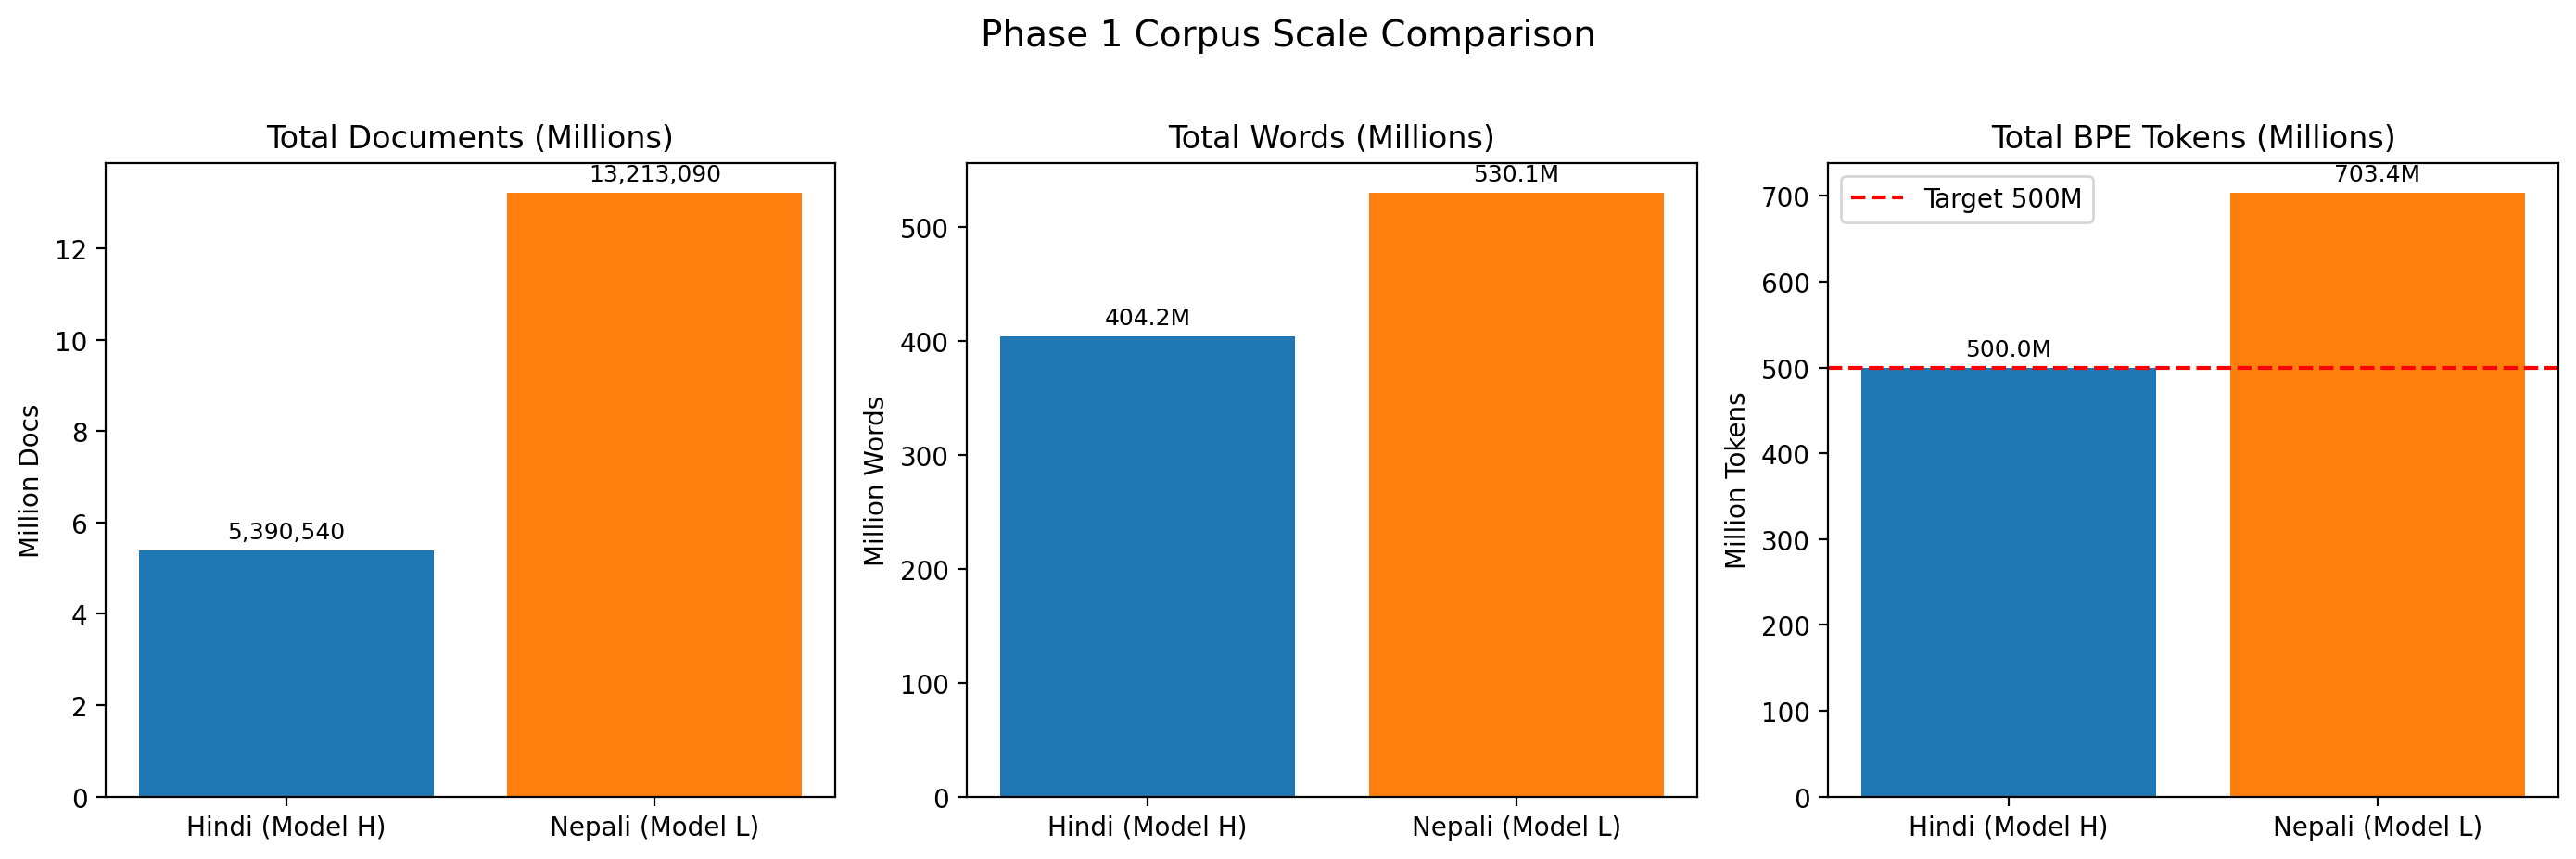
\includegraphics[width=\textwidth]{corpus_totals.png}
\caption{Corpus size comparison by documents, words, and estimated BPE tokens.}
\end{figure}

\begin{table}[H]
\centering
\caption{Document length statistics in words}
\begin{tabular}{lrrrrrrr}
\toprule
Language & Min & P50 & Mean & P90 & P95 & P99 & Max \\
\midrule
Hindi & 1 & 38 & 74.98 & 142 & 231 & 672 & 245087 \\
Nepali & 1 & 29 & 40.12 & 67 & 90 & 234 & 15776 \\
\bottomrule
\end{tabular}
\end{table}

\begin{figure}[H]
\centering
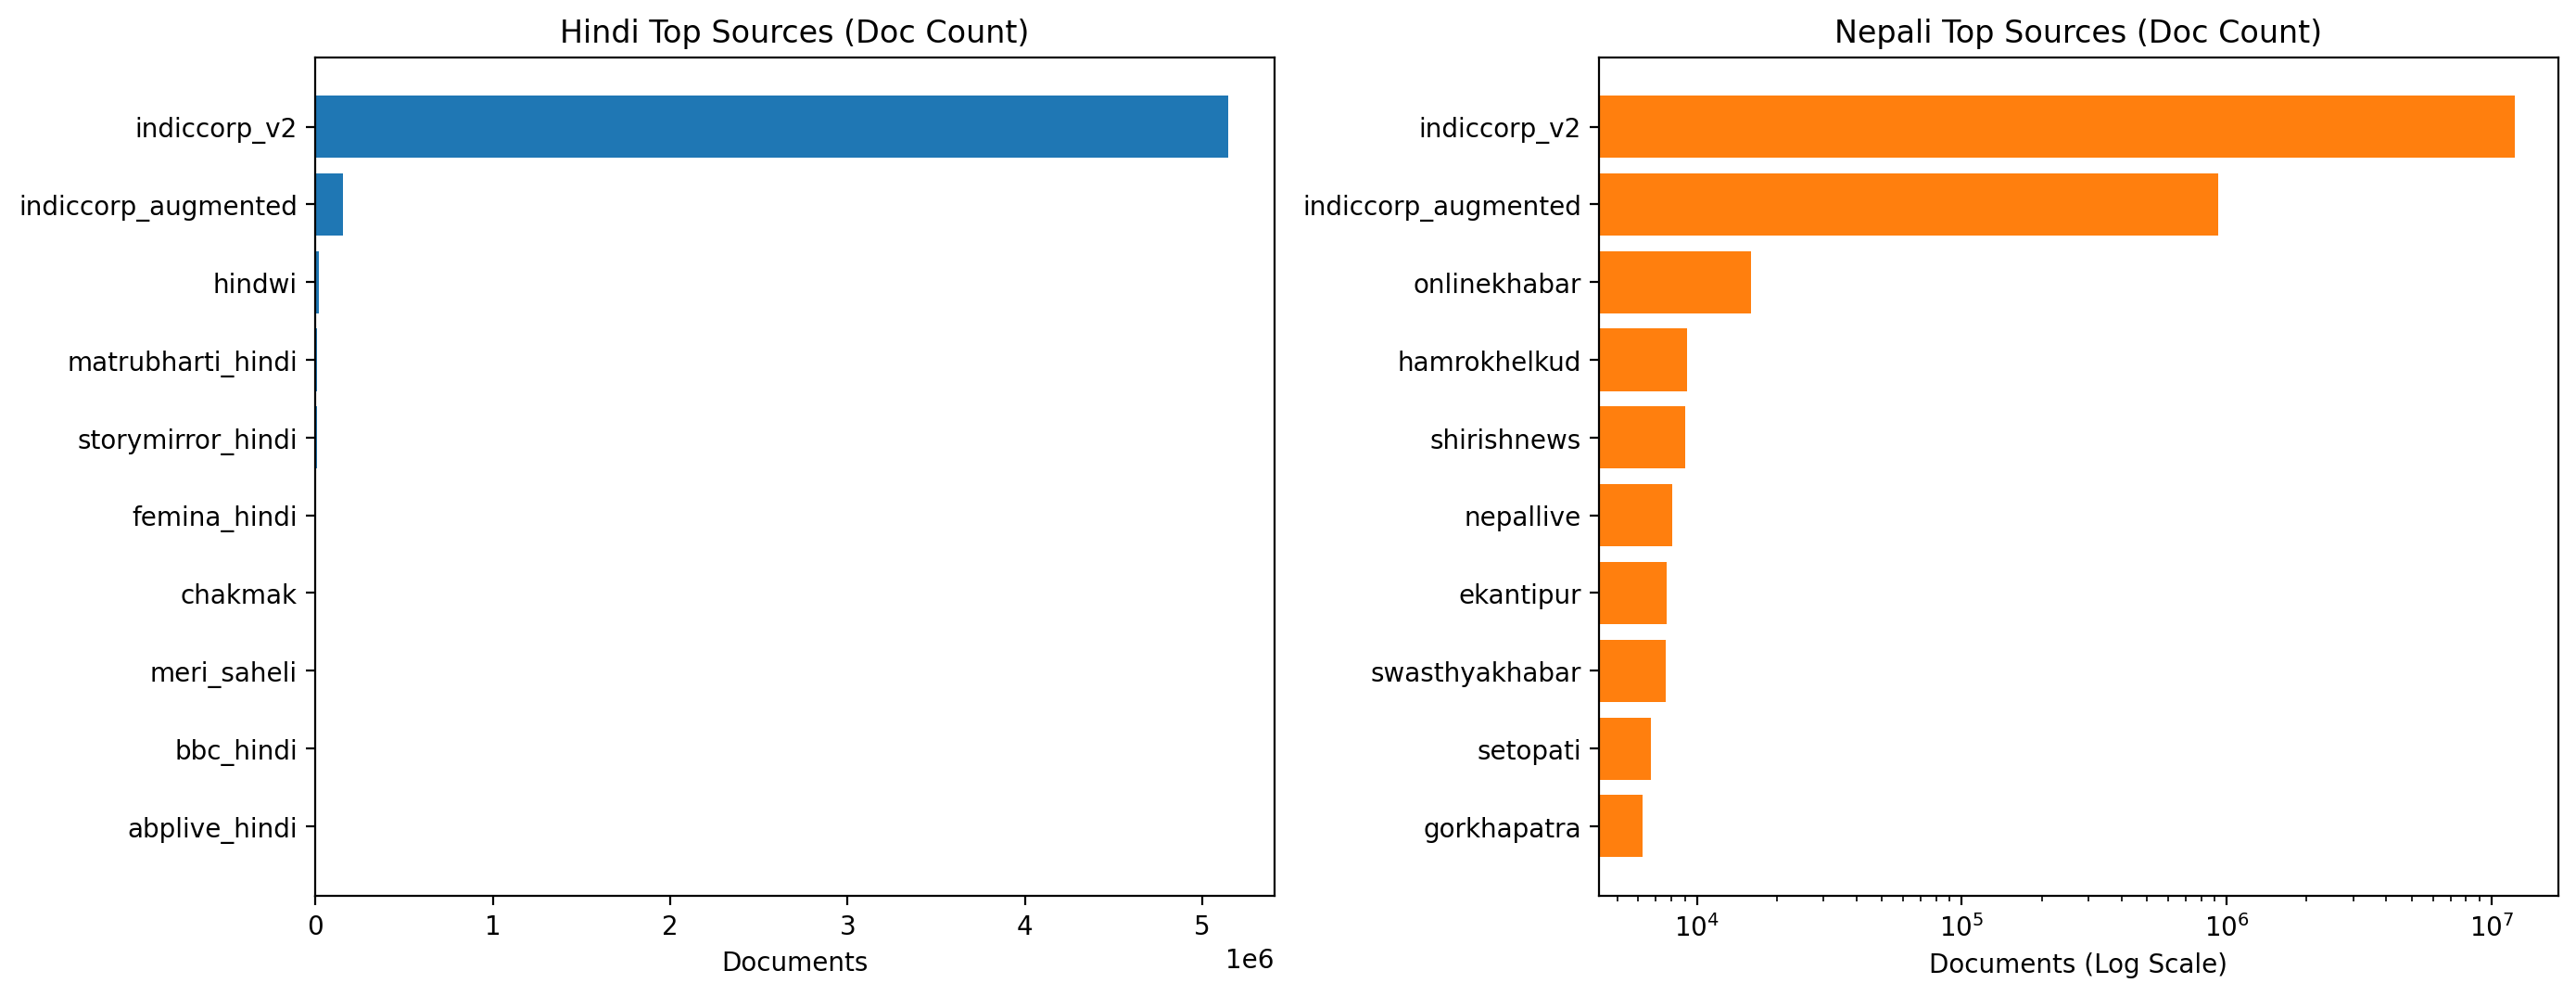
\includegraphics[width=\textwidth]{source_distribution.png}
\caption{Top source distribution by document count.}
\end{figure}

\section{Train, Validation, and Test Splits}
Splits are document-level, not sentence-level, to avoid leakage from the same
article or book segment appearing in multiple splits. The split ratio is
90\% train, 5\% validation, and 5\% test with a fixed random seed in the
preprocessing scripts.

\begin{table}[H]
\centering
\caption{Split sizes by language}
\resizebox{\textwidth}{!}{%
\begin{tabular}{lrrrr}
\toprule
Language & Split & Docs & Words & Est. BPE tokens \\
\midrule
Hindi & Train & 4,851,486 & 363,528,216 & 449,684,403 \\
Hindi & Validation & 269,527 & 20,495,877 & 25,353,399 \\
Hindi & Test & 269,527 & 20,180,238 & 24,962,954 \\
Nepali & Train & 11,891,781 & 476,919,617 & 632,872,331 \\
Nepali & Validation & 660,654 & 26,564,857 & 35,251,565 \\
Nepali & Test & 660,655 & 26,596,387 & 35,293,405 \\
\bottomrule
\end{tabular}
}
\end{table}


\section{Tokenizer Training}

\subsection{Method}
A separate custom BPE tokenizer was trained from scratch for each language
using \texttt{tokenizer/\allowbreak tokenizers.py}. The implementation uses a
Devanagari-aware regex pre-tokenizer, initializes words as character
sequences with an end-of-word marker, counts adjacent token pairs weighted by
word frequency, and repeatedly merges the highest-frequency pair using a
heap-backed pair index. Training stops when the requested merge budget is
reached or when no pair remains above the minimum frequency threshold. The
saved artifacts include a pickle model, vocabulary JSON, merges text file,
and config JSON for each language and vocabulary budget.

\subsection{Vocabulary Sweep}
Candidate BPE budgets of 5K, 10K, and 20K merges were evaluated on held-out
test splits. The realized vocabulary size can differ from the nominal merge
budget because the implementation begins with a character-level base
vocabulary and stops according to pair-frequency availability.

\begin{table}[H]
\centering
\caption{Tokenizer sweep}
\resizebox{\textwidth}{!}{%
\begin{tabular}{llrrrrr}
\toprule
Language & Tokenizer & Vocab & Fertility & Chars/token & UNK \% & Tok/s \\
\midrule
Hindi & BPE-5K & 6832 & 1.55 & 3.27 & 0.0 & 1,193,593 \\
Hindi & BPE-10K & 11263 & 1.397 & 3.63 & 0.0 & 1,060,313 \\
Hindi & BPE-20K & 20195 & 1.29 & 3.93 & 0.0 & 979,965 \\
Nepali & BPE-5K & 4777 & 1.731 & 3.73 & 0.0 & 1,019,097 \\
Nepali & BPE-10K & 9137 & 1.507 & 4.28 & 0.0 & 892,769 \\
Nepali & BPE-20K & 17973 & 1.353 & 4.77 & 0.0 & 791,549 \\
\bottomrule
\end{tabular}
}
\end{table}

\begin{figure}[H]
\centering
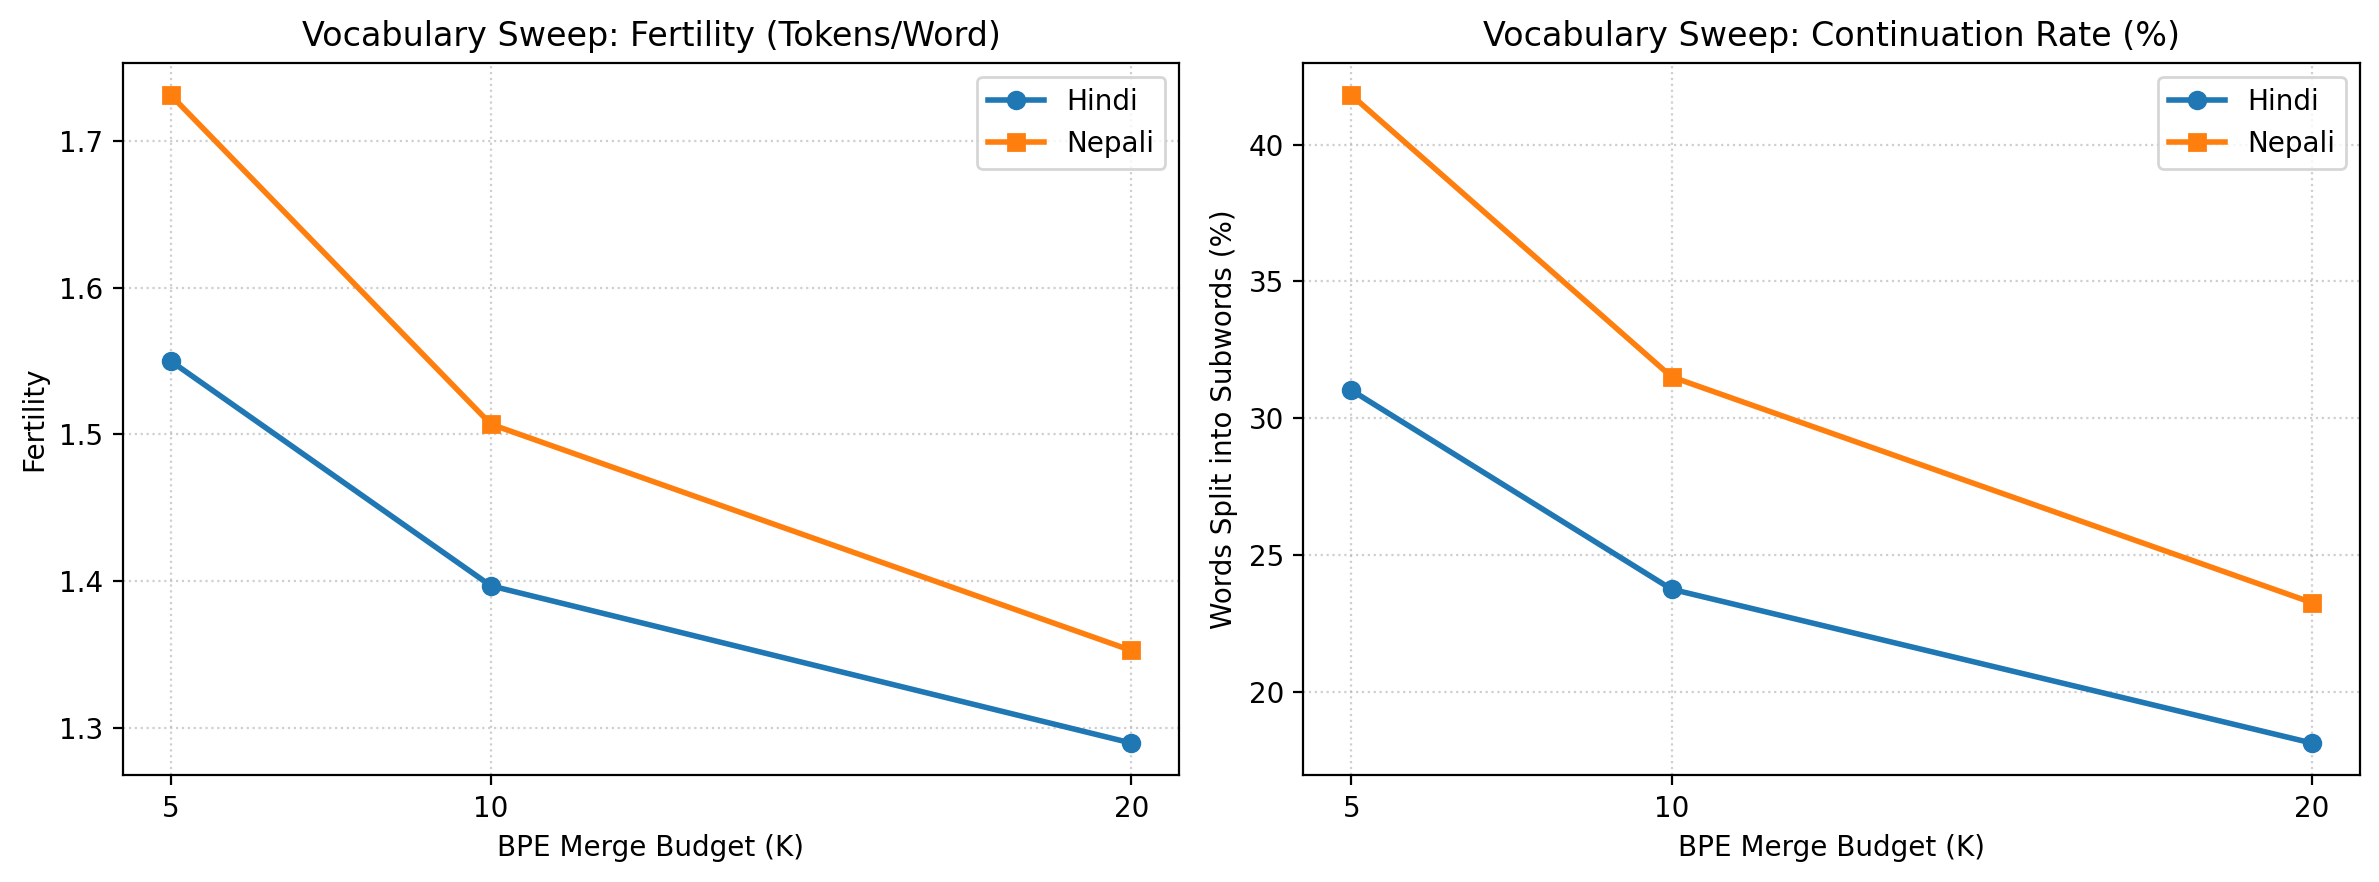
\includegraphics[width=\textwidth]{tokenizer_sweep.png}
\caption{Effect of BPE merge budget on fertility and unknown-token rate.}
\end{figure}

The 20K-budget tokenizers are selected for the next phase:
\texttt{bpe\_hi\_20000} for Hindi and \texttt{bpe\_ne\_20000} for Nepali.
They have the lowest fertility among the evaluated settings while preserving
0.00\% unknown-token rate. Hindi reaches 1.290 tokens/word with a 20,195-token
vocabulary; Nepali reaches 1.353 tokens/word with a 17,973-token vocabulary.

\subsection{Tokenization Examples}
The examples below use the selected 20K-budget tokenizers.

\begin{table}[H]
\centering
\caption{Hindi tokenization examples}
\begin{tabular}{p{0.33\textwidth}p{0.58\textwidth}}
\toprule
Input & BPE pieces \\
\midrule
\hi{भारतीय संविधान दुनिया का सबसे लंबा लिखित संविधान है।} &
\piece{भार | तीय | संविधान | दुनिया | का | सबसे | लंबा | लिखि | त | संविधान | है।} \\

\hi{भाषा मॉडल प्राकृतिक भाषा प्रसंस्करण और कृत्रिम बुद्धिमत्ता में महत्वपूर्ण भूमिका निभाते हैं।} &
\piece{भाषा | मॉडल | प्राकृतिक | भाषा | प्र | संस् | करण | और | कृ | त्रिम | बुद्धिमत्ता | में | महत्वपूर्ण | भूमिका | निभाते | हैं।} \\

\hi{प्रेमचंद की कहानियों में भारतीय ग्रामीण जीवन की वास्तविक तस्वीर देखने को मिलती है।} &
\piece{प्रेमचंद | की | कहानियों | में | भार | तीय | ग्राम | ईण | जीवन | की | वास् | तविक | तस्वीर | देखने | को | मिलती | है।} \\
\bottomrule
\end{tabular}
\end{table}

\begin{table}[H]
\centering
\caption{Nepali tokenization examples}
\begin{tabular}{p{0.33\textwidth}p{0.58\textwidth}}
\toprule
Input & BPE pieces \\
\midrule
\nep{नेपाल एक बहुजातीय, बहुभाषिक, बहुधार्मिक र बहुसांस्कृतिक विशेषतायुक्त मुलुक हो।} &
\piece{नेपाल | एक | बहु | जातीय | , | बहु | भाषिक | , | बहु | धार्मिक | र | बहु | सांस्कृतिक | विशेष | ता | युक्त | मुलुक | हो।} \\
\nep{सगरमाथा संसारको सबैभन्दा अग्लो हिमशिखर हो जुन नेपालको सोलुखुम्बु जिल्लामा पर्छ।} &
\piece{सगरमाथा | संसारको | सबैभन्दा | अग्लो | हिम | शिखर | हो | जुन | नेपालको | सोलुखु | म्बु | जिल्लामा | पर्छ।} \\
\nep{कृत्रिम बौद्धिकता र भाषा प्रविधिले मानव जीवनलाई सहज र प्रभावकारी बनाएको छ।} &
\piece{कृत्रिम | बौद्धि | कता | र | भाषा | प्रविधिले | मानव | जीवनलाई | सहज | र | प्रभावकारी | बनाएको | छ।} \\
\bottomrule
\end{tabular}
\end{table}

\subsection{Token Frequency}
The 20K-budget tokenizers produce language-appropriate high-frequency tokens.
Hindi's most frequent held-out tokens include punctuation and common
postpositions such as \piece{के}, \piece{में}, \piece{की}, \piece{से}, and
\piece{है}. Nepali's most frequent tokens include \piece{।}, comma,
\piece{र}, \piece{छ}, \piece{पनि}, \piece{को}, \piece{भएको}, and
\piece{मा}. On the test splits, the top 100 token types cover 40.17\% of
Hindi tokens and 25.99\% of Nepali tokens.

\begin{figure}[H]
\centering
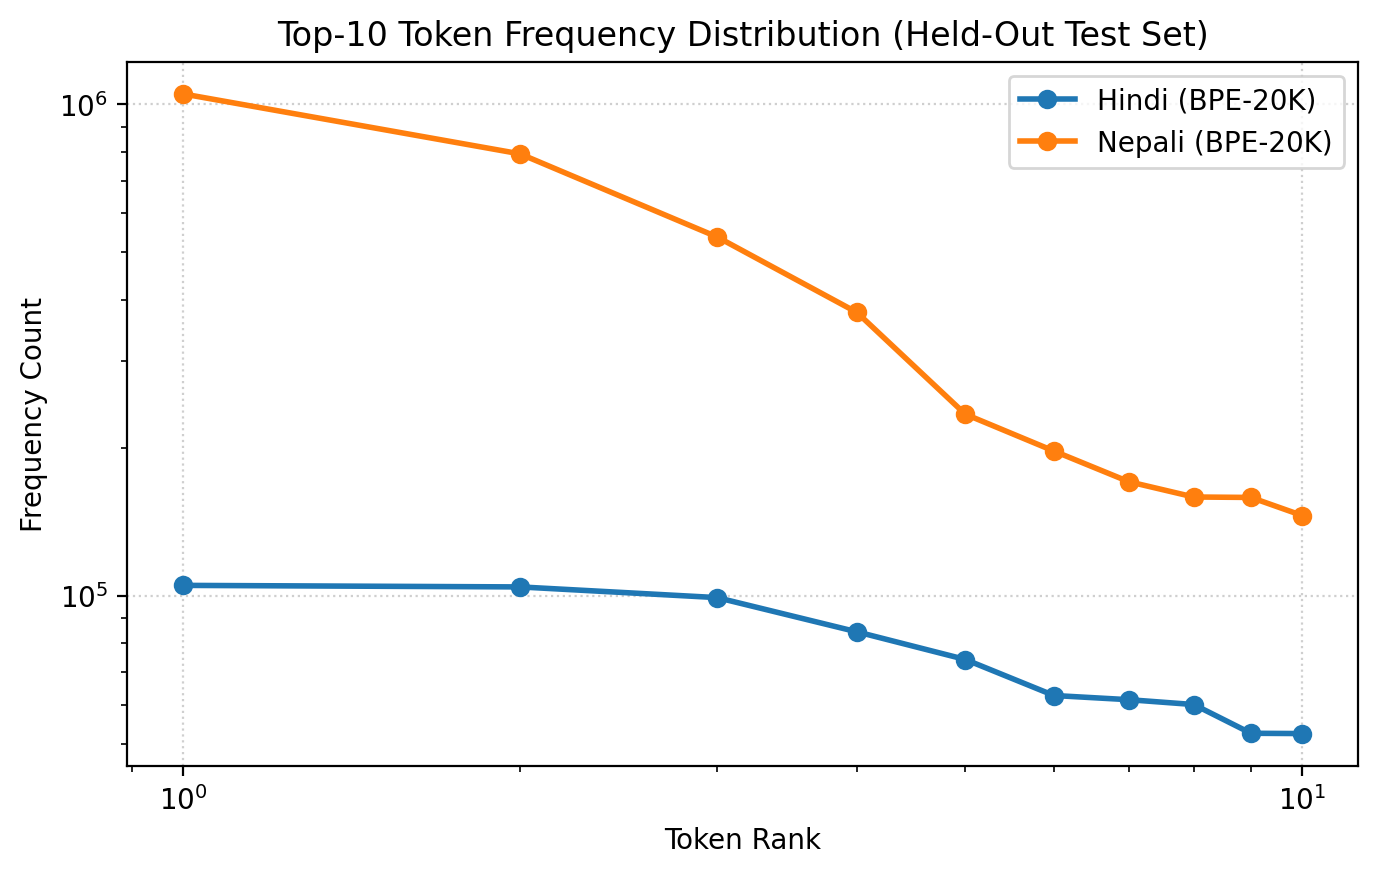
\includegraphics[width=0.82\textwidth]{token_frequency_zipf.png}
\caption{Token frequency distribution on held-out test splits.}
\end{figure}

\section{Summary}
Phase 1 produced independent Hindi and Nepali datasets, reproducible
document-level splits, source/statistics metadata, trained BPE artifacts, and
held-out tokenizer evaluations. The main technical risks for later phases are
the Nepali manual-share shortfall and the shared-script language separation
problem, both of which are visible in the report and should be addressed by
additional Nepali crawling or stricter lexical language identification before
final model training. The selected 20K-budget BPE tokenizers are ready for
Phase 2 pretraining.

\end{document}
